\documentclass[10.5pt,a4paper]{article}
\usepackage[a4paper,margin=2.2cm,top=2.3cm,bottom=2.4cm]{geometry}
\usepackage{fontspec}
\usepackage{unicode-math}
\setmainfont{TeX Gyre Pagella}
\setsansfont{Inter}[Scale=0.88]
\setmonofont{DejaVu Sans Mono}[Scale=0.80]
\setmathfont{DejaVu Math TeX Gyre}[Scale=0.95]
\usepackage{microtype}
\usepackage{xcolor}
\definecolor{accent}{HTML}{1F4E79}
\definecolor{muted}{HTML}{5F6670}
\definecolor{codebg}{HTML}{F6F7F9}
\definecolor{rule}{HTML}{D9DCE1}
\usepackage{graphicx}
\usepackage{booktabs,tabularx,array}
\usepackage{enumitem}
\setlist{nosep,leftmargin=1.4em,topsep=3pt}
\usepackage[font=small,labelfont={bf,sf},labelsep=period,skip=4pt]{caption}
\usepackage{titlesec}
\titleformat{\section}{\sffamily\large\bfseries\color{accent}}{\thesection}{0.7em}{}
\titleformat{\subsection}{\sffamily\normalsize\bfseries}{\thesubsection}{0.6em}{}
\titleformat{\subsubsection}[runin]{\sffamily\small\bfseries}{}{0em}{}[.]
\titlespacing*{\section}{0pt}{14pt}{6pt}
\titlespacing*{\subsection}{0pt}{10pt}{4pt}
\usepackage{fancyhdr}
\pagestyle{fancy}\fancyhf{}
\renewcommand{\headrulewidth}{0.4pt}
\renewcommand{\headrule}{\hbox to\headwidth{\color{rule}\leaders\hrule height \headrulewidth\hfill}}
\fancyhead[L]{\sffamily\footnotesize\color{muted}\ReportShortTitle}
\fancyhead[R]{\sffamily\footnotesize\color{muted}Eshraghi Naeini, Mohammadi}
\fancyfoot[C]{\sffamily\footnotesize\color{muted}\thepage}
\usepackage{listings}
\lstset{language=C++,basicstyle=\ttfamily\footnotesize,keywordstyle=\color{accent}\bfseries,
  commentstyle=\color{muted}\itshape,stringstyle=\color{teal!70!black},numbers=left,numberstyle=\tiny\color{muted},
  numbersep=6pt,backgroundcolor=\color{codebg},frame=single,rulecolor=\color{rule},framesep=4pt,
  xleftmargin=14pt,breaklines=true,columns=fullflexible,keepspaces=true,showstringspaces=false,
  tabsize=4,aboveskip=6pt,belowskip=6pt}
\usepackage{tikz}
\usetikzlibrary{arrows.meta,positioning,shapes.geometric,calc,fit,automata}
\tikzset{blk/.style={draw=accent,thick,fill=accent!6,rounded corners=2pt,minimum height=8mm,minimum width=20mm,align=center,font=\sffamily\small},
         io/.style={font=\sffamily\footnotesize,align=center},
         arr/.style={-{Stealth[length=2mm]},semithick},
         st/.style={state,draw=accent,thick,fill=accent!6,minimum size=9mm,font=\sffamily\footnotesize,inner sep=1pt,align=center}}
\usepackage{xurl}
\usepackage[colorlinks=true,linkcolor=accent,urlcolor=accent,citecolor=accent]{hyperref}
\usepackage{siunitx}
\sisetup{group-separator={,},group-minimum-digits=4}
\newcommand{\sig}[1]{\texttt{#1}}
\newcommand{\pass}{\textcolor{green!45!black}{\textsf{\textbf{PASS}}}}
\newcommand{\fail}{\textcolor{red!70!black}{\textsf{\textbf{FAIL}}}}
\newcommand{\prt}{\textcolor{orange!80!black}{\textsf{\textbf{PARTIAL}}}}
\newcommand{\sev}[1]{\textsf{\footnotesize\textbf{[#1]}}}
\newcommand{\repo}{https://github.com/seyedkiarash/seyedkiarash.github.io/tree/main/projects/circuit-filters-noise-cancellation}
\newcommand{\note}[1]{\par\smallskip\noindent\colorbox{accent!7}{\parbox{\dimexpr\linewidth-2\fboxsep}{\small #1}}\par\smallskip}
\setlength{\parindent}{0pt}
\setlength{\parskip}{4pt}

\newcommand{\ReportTitle}[3]{%
  \thispagestyle{plain}
  {\sffamily\small\color{muted}Circuit Theory \textbullet\ Department of Electrical Engineering, Sharif University of Technology\par}
  \vspace{2pt}
  {\sffamily\LARGE\bfseries #1\par}
  \vspace{1pt}
  {\sffamily\Large #2\par}
  \vspace{6pt}
  {\color{rule}\hrule height 0.6pt}
  \vspace{5pt}
  {\small
  \begin{tabular}{@{}l@{\hspace{2em}}l@{}}
    \textcolor{muted}{Students}  & Seyed Kiarash Eshraghi Naeini (403101383), Mohammad Sadegh Mohammadi (403102677)\\
    \textcolor{muted}{Instructor} & Dr.\ Rouhollah Amiri\\
    \textcolor{muted}{Semester} & Fall 2025 \quad\textcolor{muted}{this revision:} #3\\
    \textcolor{muted}{Tools} & LTspice, ngspice 42, MATLAB/Simulink (Simscape), Python (NumPy, SciPy, SymPy)
  \end{tabular}\par}
  \vspace{4pt}
  {\color{rule}\hrule height 0.6pt}
  \vspace{8pt}}

\newcommand{\ReportShortTitle}{Circuit Theory project -- active filters, noise cancellation, HF amplifiers}
\begin{document}
\ReportTitle{Active Filters, Analog Noise Cancellation\\and High-Frequency Amplifiers}{Circuit Theory Course Project -- Corrected and Completed Report}{October 2026}

\section*{Summary}
This report replaces the handwritten solution pages of the original submission with typed derivations.
Every result was checked again, the errors found are corrected, and the missing parts are added.
\begin{itemize}
  \item \textbf{Part I -- Sharif Analog Filter (SAF).} The transfer functions are derived from the
    node equations of the circuit as built. The design ($R_F = \SI{8}{k\ohm}$, $R_G = R_Q =
    \SI{200}{k\ohm}$) is confirmed: $f_c = \SI{19.89}{kHz}$ and $Q = 0.75$. The comparison table
    with percentage differences, which the original lacked, is added. The notch filter of the bonus
    question existed only as a screenshot; it is rebuilt as an LTspice file and simulated.
  \item \textbf{Part II -- all-pass filters and noise cancellation.}
    \begin{itemize}
      \item The 45\,\textmu s delay stage as built was not an all-pass filter. Its delay had been
        tuned by unbalancing a resistor, so its gain dropped by \SI{2}{dB} near \SI{10}{kHz}.
        The corrected values are $R_1=R_2=\SI{1.125}{k\ohm}$ and $R_3=\SI{1}{k\ohm}$: they give a
        true all-pass response (flat within \SI{0.04}{dB}) and the same \SI{45}{\micro s} delay.
      \item The delay is now verified at five test frequencies.
      \item The complete chain reduces the noise in the project audio by about \SI{33}{dB}.
    \end{itemize}
  \item \textbf{Part III -- high-frequency amplifiers.} All numerical answers of the original were
    correct, and are repeated here with the derivations typed. The two sets of plots that the
    assignment requires (Tasks 4.2 and 5.3) were missing; they are added. A more accurate common-emitter
    gain is given next to the value from the assignment's simplified formula.
\end{itemize}
Schematics, models, scripts and audio: \url{\repo}.

%=====================================================================
\part*{Part I -- Sharif Analog Filter}
\section{Transfer functions}
The SAF is a state-variable (KHN) filter: amplifier A1 forms the high-pass output $V_1$ (HP), and two
inverting integrators $R_{F1}C_1$ and $R_{F2}C_2$ produce the band-pass output $V_2$ (BP) and the
low-pass output $V_3$ (LP). The non-inverting input of A1 sees the input through $R_G$, ground
through $R_Q$ and the band-pass output through $R_4$. The inverting input sees HP through $R_2$
and LP through $R_1$. With ideal op-amps ($v_+ = v_-$, no input current):
\begin{align*}
v_+ &= \frac{V_i/R_G + V_2/R_4}{1/R_G + 1/R_Q + 1/R_4}, &
v_- &= \frac{V_1/R_2 + V_3/R_1}{1/R_1 + 1/R_2},\\
V_2 &= -\frac{V_1}{s R_{F1} C_1}, &
V_3 &= -\frac{V_2}{s R_{F2} C_2}.
\end{align*}
Solving the four equations (the algebra was also checked with SymPy) for the internal resistors $R_1=R_2$ gives three transfer functions with a common denominator
\[
D(s) = s^2 + \frac{\omega_n}{Q}s + \omega_n^2,\qquad
\omega_n = \frac{1}{\sqrt{R_{F1}R_{F2}C_1C_2}},\qquad
Q = \frac{1}{2}\left(1 + \frac{R_4}{R_G \parallel R_Q}\right)\sqrt{\frac{R_{F1}C_1}{R_{F2}C_2}},
\]
\[
H_{HP}(s) = \frac{A\,s^2}{D(s)},\qquad
H_{BP}(s) = -\frac{R_4}{R_G}\,\frac{(\omega_n/Q)\,s}{D(s)},\qquad
H_{LP}(s) = \frac{A\,\omega_n^2}{D(s)},\qquad
A = \frac{2\,(R_4\parallel R_Q)}{R_G + R_4\parallel R_Q}.
\]
The high-pass and low-pass outputs have the same pass-band gain $A$. The band-pass output is inverted, and its gain at $\omega_n$ is $-R_4/R_G$, independent of $Q$.

\section{Design for $f_c = \SI{20}{kHz}$ and $Q = 0.75$}
The assignment fixes $R_G = R_Q$ and $R_{F1}=R_{F2}=R_F$; the internal parts are $R_1=R_2=R_4=\SI{50}{k\ohm}$ and $C_1=C_2=\SI{1}{nF}$.
\begin{itemize}
  \item $f_c = 1/(2\pi R_F C) = \SI{20}{kHz}$ gives $R_F = \SI{7.958}{k\ohm}$. The nearest standard value, \SI{8}{k\ohm}, gives $f_c = \SI{19.89}{kHz}$ ($-0.5\%$).
  \item With $R_G=R_Q$, $R_G\parallel R_Q = R_G/2$, so $Q = \tfrac12(1 + 2R_4/R_G) = 0.75$ gives $R_G = 4R_4 = \SI{200}{k\ohm}$.
  \item The resulting gains are $A = 1/3$ (\SI{-9.54}{dB}) for HP and LP, and $-R_4/R_G = -0.25$ (\SI{-12.04}{dB}) for BP at $f_c$.
\end{itemize}
These are the values the team used. The design is correct.

\section{Simulation and comparison}
The LTspice schematic was simulated in two ways. Converted to ngspice, it was run with ideal op-amps and with the OP747 modelled as a single-pole amplifier ($A_0 = 10^5$, GBW = \SI{1.8}{MHz}).
The AC sweep runs from 1 to \SI{100}{kHz}. $f_c$ is the band-pass peak, and $Q = f_c/\mathrm{BW}_{-3\,\mathrm{dB}}$ is measured on the band-pass output.

\begin{table}[h]
\centering\small
\caption{Analytical and simulated SAF parameters.}\label{tab:saf}
\begin{tabular}{@{}lcccc@{}}
\toprule
Quantity & Analytical & Simulated, ideal op-amp & Simulated, GBW \SI{1.8}{MHz} & Difference (GBW) \\
\midrule
$f_c$ & \SI{19.894}{kHz} & \SI{19.894}{kHz} & \SI{20.110}{kHz} & $+1.1\%$ \\
$Q$ & 0.750 & 0.750 & 0.759 & $+1.2\%$ \\
LP gain at DC & \SI{-9.54}{dB} & \SI{-9.54}{dB} & \SI{-9.54}{dB} & 0 \\
HP gain at \SI{100}{kHz} & \SI{-9.54}{dB}\,(at $\infty$) & \SI{-9.51}{dB} & \SI{-9.17}{dB} & -- \\
BP gain at $f_c$ & \SI{-12.04}{dB} & \SI{-12.04}{dB} & \SI{-11.75}{dB} & $+0.3$\,dB \\
\bottomrule
\end{tabular}
\end{table}

\begin{figure}[h]
\centering
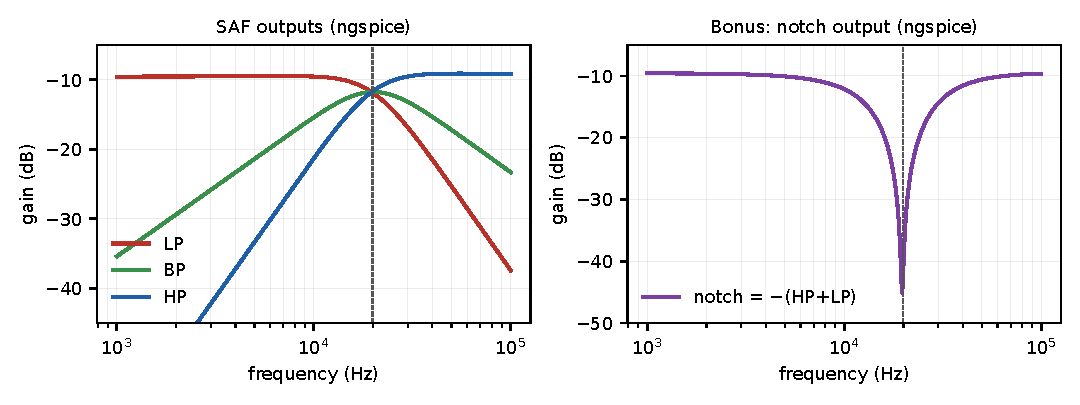
\includegraphics[width=\linewidth]{figures/saf_notch.pdf}
\caption{Left: SAF outputs (GBW model); the three curves cross at $f_c$, where $|H_{HP}|=|H_{LP}|=AQ$.
Right: notch output of the bonus circuit.}\label{fig:saf}
\end{figure}

With ideal op-amps the simulation reproduces the analysis exactly. The finite gain--bandwidth of
the op-amp adds an extra phase lag in each integrator. This raises $f_c$ and $Q$ by about 1\%,
which is the main source of difference. Resistor tolerances act on $Q$ through $R_4/(R_G\parallel R_Q)$:
a 1\% error in $R_4$, or in both $R_G$ and $R_Q$, changes $Q$ by 0.33\%. The two integrators must match ($R_{F1}C_1 =
R_{F2}C_2$) to keep the HP and LP gains equal. This is why integrated filters such as the UAF42, with laser-trimmed
internal $R_1,R_2,R_4,C_1,C_2$, are more stable than discrete builds: the critical ratios are fixed
on one die and drift together with temperature.

\section{Bonus: notch filter}
Because the HP and LP outputs have the same gain and sign, adding them cancels both numerator terms at $\omega_n$:
\[
H_N(s) = -\big(H_{HP}(s) + H_{LP}(s)\big) = -A\,\frac{s^2 + \omega_n^2}{s^2 + \frac{\omega_n}{Q}s + \omega_n^2}.
\]
A fourth op-amp in an inverting summer ($R_3=R_5=R_6=\SI{10}{k\ohm}$) adds the two outputs; this is the
circuit in the team's screenshot. Its LTspice file was missing from the submission and is rebuilt
as \texttt{saf\_notch.asc}. With ideal op-amps the notch is infinitely deep at \SI{19.89}{kHz}. With
the GBW model it reaches \SI{-45}{dB} at \SI{19.7}{kHz}, about \SI{36}{dB} below the pass band
(Fig.~\ref{fig:saf}). The team's LTspice plot shows only \SI{-35}{dB} because its linear sweep has
\SI{99}{Hz} steps and misses the bottom of the notch.

%=====================================================================
\part*{Part II -- All-Pass Filters and Analog Noise Cancellation}
\section{First-order all-pass filter}
The input reaches the non-inverting input through an $RC$ low-pass, $v_+ = V_{in}/(1+sRC)$. Because the two
$R_1$ resistors are equal, $V_{out} = 2v_+ - V_{in}$. Hence
\[
H(s) = \frac{1 - sRC}{1 + sRC},\qquad |H(j\omega)| = 1,\qquad
\angle H(j\omega) = -2\arctan(\omega RC),\qquad
\tau_g(\omega) = \frac{2RC}{1 + (\omega RC)^2}.
\]
The pole and zero are mirror images, so the magnitude is 1 at every frequency. The phase falls from
$0^\circ$ at DC through $-90^\circ$ at $\omega = 1/RC$ to $-180^\circ$. A sine passes with its amplitude unchanged and
is delayed by $\tau_g$; low frequencies are delayed by $2RC$. The product $RC$ alone fixes the frequency of any given phase
shift. For example, $\omega_{90^\circ} = 1/RC$; $R_1$ only has to be matched.

\section{Second-order all-pass filter (the delay stage)}
\subsection{Transfer function of the circuit as built}
In the team's circuit (Fig.~4 of the assignment), op-amp U1 with $C_1$, $C_2$, $R_1$ and $R_2$ forms a
second-order section. U2 sums $-(R_{42}/R_3)\,v_{U1}$ and $-(R_{42}/R_{41})\,v_{in}$. Solving the node equations gives
\[
H(s) = -\frac{R_{42}}{R_{41}}\cdot
\frac{C_1C_2R_1R_2\,s^2 + \big[R_1(C_1+C_2) - C_1R_2\,R_{41}/R_3\big]s + 1}
     {C_1C_2R_1R_2\,s^2 + R_1(C_1+C_2)\,s + 1}.
\]
The denominator gives $\omega_0 = 1/\sqrt{R_1R_2C_1C_2}$ and $Q = \sqrt{R_2/R_1}\cdot\sqrt{C_1C_2}/(C_1+C_2)$.
Unlike the first-order section, the second-order one has two parameters, $\omega_0$ and $Q$, so the steepness of the phase transition can be set as well as its frequency.
The response is all-pass only if the middle coefficient of the numerator is the negative of
that of the denominator, and $R_{42}=R_{41}$ for unit gain. With $C_1=C_2=C$ and $R_1=R_2=R$:
\[
\frac{R_{41}}{R_3} = 4 \quad\Longrightarrow\quad H(s) = -\left(\frac{1 - sRC}{1 + sRC}\right)^2,\qquad
\angle H = 180^\circ - 4\arctan(\omega RC),\qquad \tau_g(0) = 4RC.
\]
This equal-component section has a double real pole ($Q = 1/2$). It behaves like two first-order sections in series, with twice the phase shift and twice the delay. The leading minus sign is the phase inversion that the noise-cancelling chain uses.

\subsection{Error in the original values and correction}
The team built the stage with $R_1=R_2=\SI{1.25}{k\ohm}$, $C=\SI{10}{nF}$, $R_3=\SI{1.125}{k\ohm}$ and
$R_{41}=R_{42}=\SI{4}{k\ohm}$. Then $R_{41}/R_3 = 3.56 \neq 4$, so the numerator is not the mirror
image of the denominator. The low-frequency delay came out at the required \SI{45}{\micro s}
($\tau_g(0) = (R_{41}/R_3)\,RC = 3.56 \times \SI{12.5}{\micro s} = \SI{44.4}{\micro s}$) only because the all-pass condition was broken. As a result, the gain falls by \SI{2.1}{dB} near
\SI{10}{kHz} (Fig.~\ref{fig:apfix}). The correct design keeps the all-pass condition and sets the delay through $RC$:
\[
4RC = \SI{45}{\micro s} \;\Rightarrow\; RC = \SI{11.25}{\micro s} \;\Rightarrow\;
R_1 = R_2 = \SI{1.125}{k\ohm}\ (C = \SI{10}{nF}),\qquad R_3 = R_{41}/4 = \SI{1}{k\ohm}.
\]
The two numbers \SI{1.125}{k\ohm} and \SI{1}{k\ohm} had evidently been placed in the wrong positions. The corrected
schematic is \texttt{stage3\_allpass\_delay\_45us\_corrected.asc}. The same values are corrected in the
Simulink model (\texttt{anc\_system\_corrected.slx}).

\begin{figure}[h]
\centering
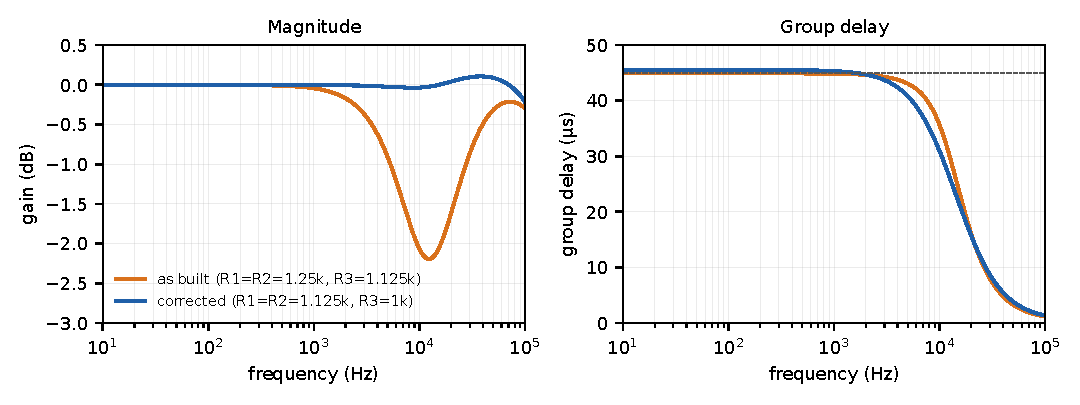
\includegraphics[width=\linewidth]{figures/allpass_fix.pdf}
\caption{Delay stage, ngspice with the OP747 GBW model. As built, the magnitude is not flat; corrected, it stays within
\SI{0.04}{dB} up to \SI{20}{kHz}, and the delay stays at \SI{45}{\micro s} up to about \SI{3}{kHz}.}\label{fig:apfix}
\end{figure}

\subsection{Verification of the delay}
Each stage was driven with a \SI{1}{V} sine. The delay is the time between rising zero crossings of the input and the
inverted output (Fig.~\ref{fig:tran}), and the amplitude ratio is measured on the same waveforms.

\begin{table}[h]
\centering\small
\caption{Transient test of the delay stage (ngspice, GBW model).}\label{tab:delay}
\begin{tabular}{@{}rcccc@{}}
\toprule
& \multicolumn{2}{c}{As built} & \multicolumn{2}{c}{Corrected}\\
\cmidrule(lr){2-3}\cmidrule(l){4-5}
Frequency & Delay & Amplitude ratio & Delay & Amplitude ratio\\
\midrule
\SI{200}{Hz} & \SI{44.9}{\micro s} & 1.000 & \SI{45.5}{\micro s} & 1.000\\
\SI{500}{Hz} & \SI{44.9}{\micro s} & 0.999 & \SI{45.5}{\micro s} & 1.000\\
\SI{1}{kHz} & \SI{44.9}{\micro s} & 0.995 & \SI{45.5}{\micro s} & 1.000\\
\SI{2}{kHz} & \SI{44.8}{\micro s} & 0.981 & \SI{45.3}{\micro s} & 0.999\\
\SI{5}{kHz} & \SI{44.3}{\micro s} & 0.901 & \SI{43.9}{\micro s} & 0.997\\
\bottomrule
\end{tabular}
\end{table}
With ideal op-amps the corrected stage gives exactly \SI{45.0}{\micro s} at low frequency; the op-amp bandwidth adds \SI{0.5}{\micro s}.

\begin{figure}[h]
\centering
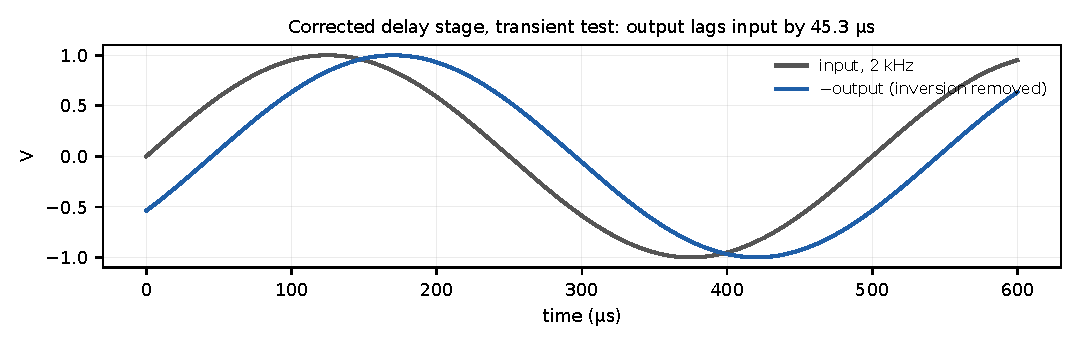
\includegraphics[width=\linewidth]{figures/delay_transient.pdf}
\caption{Corrected delay stage with a \SI{2}{kHz} input.}\label{fig:tran}
\end{figure}

\section{Higher-order all-pass filters}
Cascading $N$ sections multiplies their responses. The magnitude stays 1, the phases add, and so do the group delays
(a cascade of $N$ first-order sections has $\tau_g(0) = 2NRC$). The impulse response of one first-order section is
$h(t) = -\delta(t) + \frac{2}{RC}e^{-t/RC}u(t)$: an impulse followed by a single exponential. For a cascade
the impulse response is the convolution of the sections' responses. Its energy moves to later times, near
the group delay, and it acquires alternating lobes, because the phase now changes quickly with frequency (Fig.~\ref{fig:apth}).
\begin{itemize}
  \item \textbf{Order and duration.} The duration of the impulse response grows roughly in proportion to the order.
  \item \textbf{Phase.} The total phase shift grows by $180^\circ$ for each first-order section ($360^\circ$ for each second-order one).
  \item \textbf{Visual difference.} A 10th-order response is a long, ringing burst centred near $\tau_g$, whereas a 1st-order response is a single spike and decay.
\end{itemize}
\begin{figure}[h]
\centering
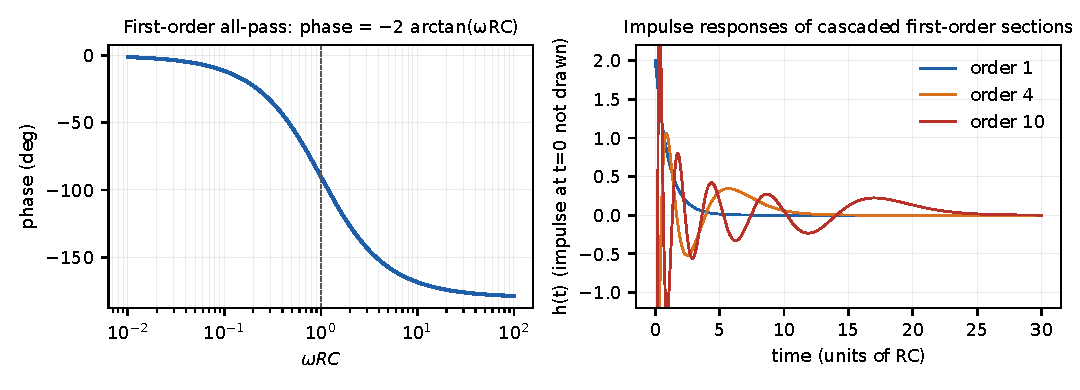
\includegraphics[width=\linewidth]{figures/allpass_theory.pdf}
\caption{Left: phase of a first-order section. Right: impulse responses of cascades of 1, 4 and 10 equal sections (the initial $\pm\delta$ term is not drawn).}\label{fig:apth}
\end{figure}

\section{Analog noise cancellation}
\subsection{Why a delay is needed}
The reference microphone picks up the noise before it reaches the listener. The acoustic path to the
point of cancellation, and the electronics themselves, delay the noise that has to be cancelled. The
anti-noise must arrive at the same time and with opposite sign. A phase error $\varphi$ leaves a
residual of $2|\sin(\varphi/2)|$ times the noise, so even $\varphi = 10^\circ$ limits the reduction to about \SI{15}{dB}.
The delay stage therefore aligns the anti-noise in time with the noise it cancels.

\subsection{The three stages}
\begin{enumerate}
  \item \textbf{Gain of 10.} A non-inverting amplifier with $R_f=\SI{9}{k\ohm}$ and $R_g=\SI{1}{k\ohm}$, so $1 + R_f/R_g = 10$. A \SI{1}{V} test sine gives \SI{10}{V}.
  \item \textbf{Delay.} The corrected all-pass stage above: \SI{45}{\micro s}, gain $-1$.
  \item \textbf{Combination.} The assignment asks for a subtractor. Because the delay stage already
    inverts the noise, the team instead used an inverting summer ($\SI{1}{k\ohm}$ resistors) followed by an
    inverter, so the output is music $+$ noise $-$ delayed noise. This is equivalent to a subtractor. With
    test inputs of \SI{1}{V} and \SI{2}{V} the output is \SI{3}{V}, as expected.
\end{enumerate}

\subsection{System results}
The chain was built in Simulink (Simscape: band-limited op-amps with $A=2\times10^5$ and resistors) and driven with the two recordings.
The noise inside the recording is $10.06$ times the isolated noise and lags it by about \SI{30}{\micro s};
this was found by a least-squares fit, which also gives an estimate of the clean music.
\begin{itemize}
  \item \textbf{Simulink output, original values:} noise reduced by \SI{33.3}{dB}; signal-to-noise ratio from \SI{8.4}{dB} to \SI{41.6}{dB} (Fig.~\ref{fig:anc}).
  \item \textbf{Corrected values:} a Python model of the same transfer functions gives \SI{33.3}{dB}. The model reproduces the Simulink output to within 0.5\%. The correction leaves the result unchanged because the noise lies below \SI{2}{kHz}, where both versions of the stage are nearly ideal.
  \item \textbf{Limiting factor:} the mismatch between the specified \SI{45}{\micro s} and the \SI{30}{\micro s} delay present in the recordings.
    With $RC = \SI{7.5}{\micro s}$ ($R_1=R_2=\SI{750}{\ohm}$) the same circuit would reduce the noise by about \SI{44}{dB}.
\end{itemize}

\begin{figure}[h]
\centering
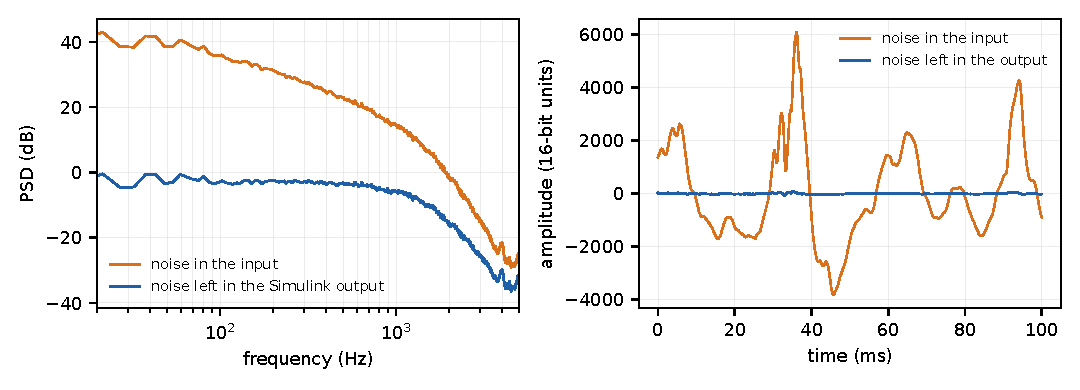
\includegraphics[width=\linewidth]{figures/anc.pdf}
\caption{Noise before and after the cancellation chain (Simulink output).}\label{fig:anc}
\end{figure}

%=====================================================================
\part*{Part III -- High-Frequency Response of Transistor Amplifiers}
\section{Model parameters (Tasks 1 and 2)}
\begin{table}[h]
\centering\small
\caption{Small-signal parameters.}\label{tab:par}
\begin{tabular}{@{}lr@{\hspace{2.5em}}lr@{}}
\toprule
\multicolumn{2}{@{}c}{MOSFET} & \multicolumn{2}{c@{}}{BJT}\\
\midrule
$g_m = 2I_D/V_{OV}$ & \SI{4.0}{mA/V} & $g_m = I_C/V_T$ & \SI{80}{mA/V}\\
$r_o = V_A/I_D$ & \SI{40}{k\ohm} & $r_\pi = \beta_0/g_m$ & \SI{1.5}{k\ohm}\\
$C_{gs} = (\tfrac23 WL + WL_{ov})C_{ox}$ & \SI{59.7}{fF} & $r_o = V_A/I_C$ & \SI{37.5}{k\ohm}\\
$C_{gd} = WL_{ov}C_{ox}$ & \SI{6.4}{fF} & $C_\pi = \tau_F g_m + 2C_{je0}$ & \SI{5.20}{pF}\\
 & & $C_\mu = C_{\mu0}/(1+V_{CB}/V_{0c})^m$ & \SI{0.125}{pF}\\
\bottomrule
\end{tabular}
\end{table}
The three expressions for $g_m$ in Eq.~(2) agree: $\mu_nC_{ox}(W/L)V_{OV} = 400\mu\cdot 40\cdot 0.25 = \SI{4}{mA/V}$.

\section{Unity-gain frequency (Tasks 3 and 4)}
\textbf{MOSFET.} With the drain shorted, KCL at the drain gives $I_o = (g_m - sC_{gd})V_{gs}$, and at the gate
$I_i = s(C_{gs}+C_{gd})V_{gs}$. Hence
\[
A_i(s) = \frac{g_m - sC_{gd}}{s(C_{gs}+C_{gd})} \approx \frac{g_m}{s(C_{gs}+C_{gd})}\ \ (g_m \gg \omega C_{gd}),
\qquad f_T = \frac{g_m}{2\pi(C_{gs}+C_{gd})} = \SI{9.63}{GHz}.
\]
\textbf{BJT.} With the collector shorted, $I_b = (1/r_\pi + s(C_\pi+C_\mu))V_\pi$ and $I_c = (g_m - sC_\mu)V_\pi$. Hence
\[
h_{fe}(s) = \frac{g_m - sC_\mu}{1/r_\pi + s(C_\pi+C_\mu)} \approx \frac{\beta_0}{1 + s/\omega_\beta},\qquad
\beta_0 = g_m r_\pi,\quad \omega_\beta = \frac{1}{r_\pi(C_\pi+C_\mu)}.
\]
$|h_{fe}(j\omega_T)| = 1$ gives $\omega_T = \omega_\beta\sqrt{\beta_0^2-1} \approx \beta_0\omega_\beta = g_m/(C_\pi+C_\mu)$.
The base resistance $r_x$ does not affect $h_{fe}$, because the base is driven by a current source.
Numerically, $f_\beta = \SI{19.9}{MHz}$ and $f_T = \SI{2.39}{GHz} = \beta_0 f_\beta$. The exact expressions, including the right-half-plane zeros, cross 0\,dB at \SI{9.67}{GHz} and \SI{2.39}{GHz}.

\begin{figure}[h]
\centering
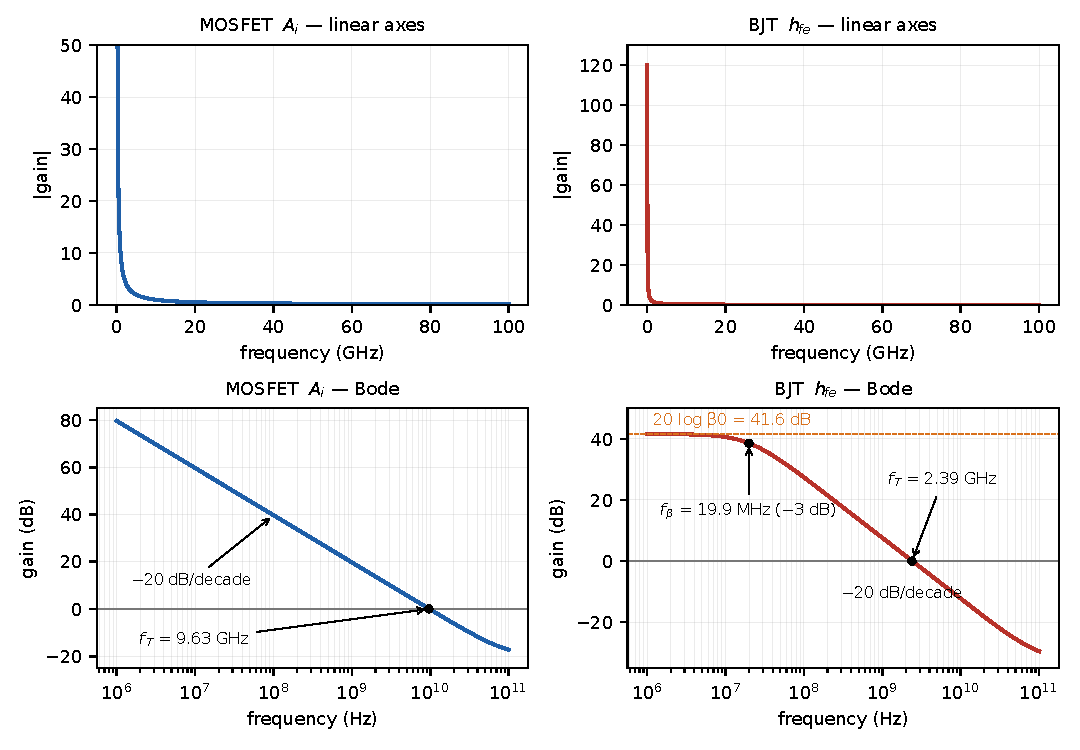
\includegraphics[width=0.92\linewidth]{figures/current_gain.pdf}
\caption{Short-circuit current gain from \SI{1}{MHz} to \SI{100}{GHz} (Task 4.2), on linear axes and as Bode plots.}\label{fig:cg}
\end{figure}

On linear axes (top of Fig.~\ref{fig:cg}) nearly all of the decade-wide frequency range is squeezed against the axis.
$f_\beta$ and $f_T$ cannot be read there, and the $1/f$ behaviour looks like a sudden drop. The Bode plot turns a
single-pole roll-off into a straight line of $-20$\,dB/decade. Then $f_T$ is the 0\,dB crossing, $f_\beta$ is
the point \SI{3}{dB} below $20\log\beta_0 = \SI{41.6}{dB}$, and many decades are visible at once. That is why
frequency responses are drawn as Bode plots.

\section{CS and CE amplifiers (Task 5)}
For the CS stage,
\begin{gather*}
A_v(s) = \frac{A_M}{1 + s/\omega_H},\qquad
A_M = -\frac{R_G}{R_G+R_{sig}}\,g_m R_L',\qquad R_L' = r_o\parallel R_D\parallel R_L,\\
\omega_H = \frac{1}{(R_{sig}\parallel R_G)\,[C_{gs} + C_{gd}(1+g_mR_L')]}.
\end{gather*}

\begin{table}[h]
\centering\small
\caption{Amplifier results (Task 5.2).}\label{tab:amp}
\begin{tabular}{@{}lcc@{}}
\toprule
 & CS (MOSFET) & CE (BJT, $r_x=\SI{100}{\ohm}$)\\
\midrule
$R_L'$ & \SI{4.44}{k\ohm} & \SI{2.34}{k\ohm}\\
$A_M$ & $-17.7$ (\SI{24.9}{dB}) & $-25.5$ (\SI{28.1}{dB})\\
$C_{in}$ & \SI{180}{fF} & \SI{28.7}{pF}\\
$R_{sig}'$ & \SI{49.8}{k\ohm} & \SI{1.36}{k\ohm}\\
$f_H$ & \SI{17.8}{MHz} & \SI{4.08}{MHz}\\
GBW $=|A_M|f_H$ & \SI{314}{MHz} & \SI{104}{MHz}\\
0\,dB crossing (plot) & \SI{314}{MHz} & \SI{104}{MHz}\\
\bottomrule
\end{tabular}
\end{table}

The Miller term dominates both input capacitances: $C_{gd}(1+g_mR_L') = \SI{120}{fF}$ against $C_{gs} = \SI{60}{fF}$, and $C_\mu(1+g_mR_L') = \SI{23.5}{pF}$ against $C_\pi = \SI{5.2}{pF}$.

\note{The CE formulas in the assignment apply the input divider to $r_x + r_\pi$. Only the part across $r_\pi$
drives $g_m$, so the exact mid-band gain contains a further factor $r_\pi/(r_x+r_\pi) = 0.94$:
$A_M = -23.9$ (\SI{27.6}{dB}). Likewise, the resistance seen by $C_{in}$ is $r_\pi \parallel (r_x + R_{sig}\parallel R_B) = \SI{1.29}{k\ohm}$,
so $f_H = \SI{4.30}{MHz}$. The table follows the assignment's formulas, as the task requires.}

\begin{figure}[h]
\centering
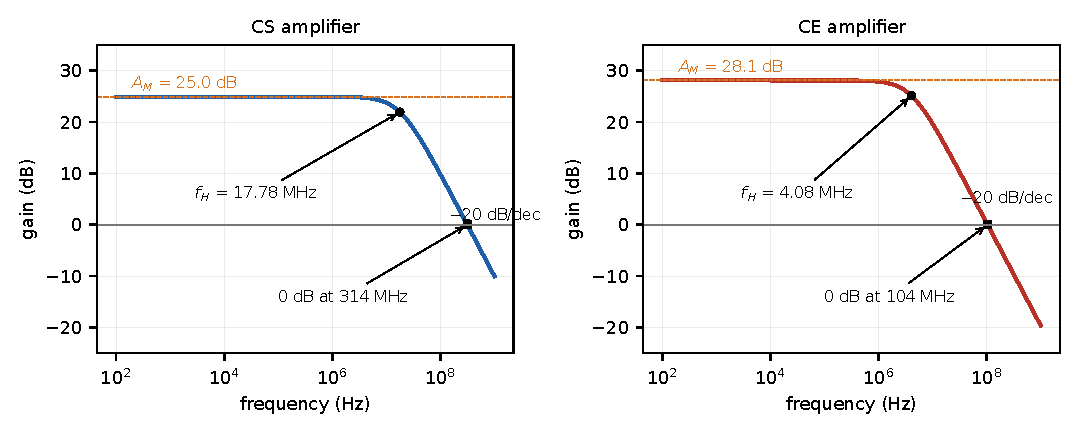
\includegraphics[width=\linewidth]{figures/amplifiers.pdf}
\caption{Bode plots of the two amplifiers from \SI{100}{Hz} to \SI{1}{GHz} (Task 5.3).}\label{fig:amp}
\end{figure}

In both plots (Fig.~\ref{fig:amp}) the gain is \SI{3}{dB} below mid-band at $f_H$ and then falls at $-20$\,dB/decade. Hence the
0\,dB crossing equals $|A_M| f_H$. For a single-pole response the gain-bandwidth product is constant, and it equals the unity-gain frequency.

\section{RF input matching (Task 6)}
With inductive degeneration, $Z_{in} = sL_g + g_mL_s/C_{gs} + 1/(sC_{gs})$.
\begin{itemize}
  \item The real part is $g_mL_s/C_{gs} = \SI{50}{\ohm}$, which gives $L_s = 50\,C_{gs}/g_m$. Since $g_m/C_{gs} \approx \omega_T$, this is $L_s \approx 50/\omega_T$; for the MOSFET above, $L_s = \SI{0.75}{nH}$.
  \item Cancelling the imaginary part at $\omega_0$, $\omega_0L_g - 1/(\omega_0C_{gs}) = 0$, gives $L_g = 1/(\omega_0^2C_{gs})$.
\end{itemize}

With an inductive load, $A_v = -g_m Z_L$ becomes complex and changes rapidly near the tank resonance. The
component that links output to input is $C_{gd}$, whose Miller admittance is $sC_{gd}(1 - A_v)$.
\begin{itemize}
  \item Below resonance the load is inductive, $A_v$ has a positive imaginary part, and the Miller term contributes a
    \emph{negative} real part to the input admittance. Above resonance it adds capacitance.
  \item The equivalent capacitance $C_{eq} = C_{gd}(1-A_v)$ is therefore complex and can have a negative real part.
  \item A negative input conductance can cancel the source conductance, which can make the stage oscillate. This is why tuned stages use cascodes or neutralisation to remove the $C_{gd}$ feedback.
\end{itemize}

\section{Tuned amplifier with a transformer load (Task 7)}
The load is the parallel combination $Z = R_{total}\parallel sL_p \parallel 1/(sC_{out})$, so
\[
A_v(s) = -g_m\,\frac{s/C_{out}}{s^2 + s/(R_{total}C_{out}) + 1/(L_pC_{out})}.
\]
\begin{itemize}
  \item This is a band-pass response: it has a zero at DC, where the inductor shorts the output, and two zeros at infinity, where the capacitor does.
  \item The gain peaks at $\omega_0 = 1/\sqrt{L_pC_{out}}$. There the $s^2$ and constant terms cancel, which leaves the real value $A_v(j\omega_0) = -g_mR_{total}$.
  \item With $Q = R_{total}\,\omega_0C_{out}$, the bandwidth is $\mathrm{BW} = \omega_0/Q = 1/(R_{total}C_{out})$, independent of $L_p$.
\end{itemize}
The peak gain is proportional to $R_{total}$ and the bandwidth inversely, so their product $g_m/C_{out}$ is fixed. A higher gain can only be bought with a narrower band.

\section*{Files}
\begin{itemize}
  \item \texttt{part1-state-variable-filter/}: \texttt{state\_variable\_filter.asc} and \texttt{saf\_notch.asc} (rebuilt).
  \item \texttt{part2-allpass-noise-cancellation/ltspice/}: gain, summer/inverter and delay stages, as built and corrected.
  \item \texttt{part2-allpass-noise-cancellation/simulink/}: \texttt{anc\_system.slx} (as submitted) and\\ \texttt{anc\_system\_corrected.slx}.
  \item \texttt{verification/}: ngspice netlists, \texttt{anc\_check.py}, and the scripts for the figures of this report.
\end{itemize}
\end{document}
